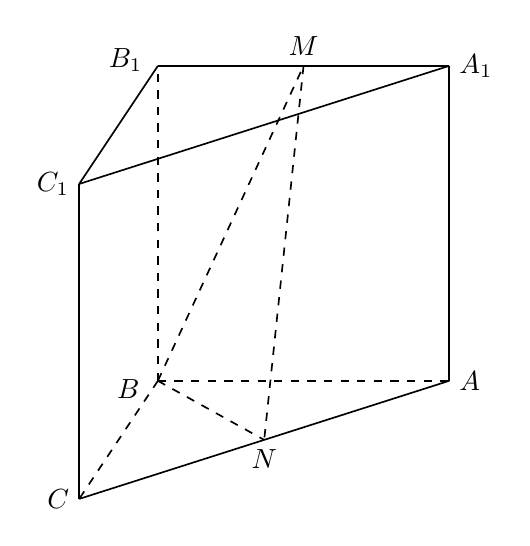
\begin{tikzpicture}[line width=0.6pt, font=\normalsize]
\coordinate (B) at (1.5,1.5);
\coordinate (A) at (5.2000000000,1.5000000000);
\coordinate (C) at (0.5,0);
\coordinate (N) at (2.8500000000,0.7500000000);
\coordinate (B1) at (1.5000000000,5.5000000000);
\coordinate (A1) at (5.2000000000,5.5000000000);
\coordinate (C1) at (0.5000000000,4.0000000000);
\coordinate (M) at (3.3500000000,5.5000000000);
% bottom face: C-A solid with N, B-A/B-C dashed
\draw (C) -- (A);
\draw[dashed] (B) -- (A);
\draw[dashed] (B) -- (C);
\draw[dashed] (B) -- (N);
% verticals
\draw[dashed] (B) -- (B1);
\draw (A) -- (A1);
\draw (C) -- (C1);
% top face
\draw (B1) -- (A1);
\draw (A1) -- (C1);
\draw (B1) -- (C1);
% segments BM, MN, BN
\draw[dashed] (B) -- (M);
\draw[dashed] (M) -- (N);
\node[below left,xshift=-3pt,yshift=4pt] at (B) {$B$};
\node[right] at (A) {$A$};
\node[left] at (C) {$C$};
\node[below] at (N) {$N$};
\node[left,xshift=-2pt,yshift=2pt] at (B1) {$B_{1}$};
\node[right] at (A1) {$A_{1}$};
\node[left] at (C1) {$C_{1}$};
\node[above] at (M) {$M$};
\end{tikzpicture}
